\documentclass[conference]{IEEEtran}
%\usepackage{draftwatermark}
\usepackage{graphicx}
\usepackage{cite}
\usepackage[belowskip=-10pt,aboveskip=2pt]{caption}
\usepackage[cmex10]{amsmath}
\usepackage{tikz}
\usepackage{csquotes}
\usetikzlibrary{patterns}
\usetikzlibrary{positioning}
\usetikzlibrary{arrows}
\usetikzlibrary{decorations.markings}
\newcommand{\todocomment}[2]{{\bf\sc (* from #1: #2 *) }}

\begin{document}

\title{Behavior Identification and Predictive Analysis of Philadelphia Parking Authority Agents}

\author{
\IEEEauthorblockN{Dustin~S.~Ingram}
\IEEEauthorblockA{Department of Computer Science\\
Drexel University, Philadelphia, PA\\
Email: dustin@cs.drexel.edu}
}

\maketitle

\begin{abstract}
In this project, I will use and compare various machine learning techniques in
an attempt to discover spatio-temporal patterns within time-coded location-based
data on Philadelphia parking ticket data. I will attempt to use the found
patterns to build a predictive model for the most probably current location of
an agent at a given day and time, as well as identify interesting
characteristics and behaviors within the data.

\end{abstract}

\section{Related Work and Novelty}
\label{sec:intro}
Finding patterns in movement data is a problem that has roots in a diverse array
of problem sets, from searching for suggestions for improvements of public and
mass transit in pedestrian, to analysis of traffic bottlenecks or travel
patterns based on driver data~\cite{holyoakAUS}, to using shopper data to reveal
commonalities in the way that people visit a given area~\cite{Orellana2012672},
to analyzing the movements of herds of animals~\cite{zebranet}~\cite{animaleda}.

This paper will attempt to use machine learning to perform a spatio-temporal
analysis of a body of data which consists of a large portion of parking ticket
data for the City of Philadelphia, spanning the months of December, January and
February, using .

The Philadelphia Parking Authority distributes over three thousand tickets per
day over a broad geographical area which comprises the metropolitan area of
Philadelphia for a variety of infractions. There has been little to no
publicly available analysis of the behavior or effectiveness of patterns of
such individual agents, either in Philadelphia or other cities, and the
applications can span over a broad area of activity, including mail and parcel
delivery, door-to-door canvassing, and more.

\begin{figure}[h]
\small{\texttt{\{"\_id" : 58686207, "resolved" : false, "violation" : "METER
EXPIRED CC", "issueTime" : ISODate("2013-02-09T17:02:00Z"), "violationCode" :
"1210051 C", "location" : "300 BLK SOUTH ST SS"\}}
\caption{A sample of individual ticket data.}}
\end{figure}

\section{Approach}
\label{sec:approach}
The approach will be to collect data and process it, including performing the
necessary geo-coding, which requires building a data-collection system and
corresponding database for storing the retrieved data. Then, the data will be
given a preliminary evaluation based on the amount collected at time, and may be
limited to a certain geographic area. Because the data is discretized at the
per-block level, it is a prime candidate for use with a Hidden Markov Model, as
there is a number of distinct data points with very accurate corresponding
time-stamps, however on the general path, there may be points missing from one
day to the other which can be filled in using the model. In addition, various
known techniques for sequential pattern mining can be
applied~\cite{Agrawal95miningsequential}.

From~\cite{Dodge:2008:TTM:1594710.1594716}:
\blockquote{\textbf{Co-location in space:} Occurs when the trajectories of
moving objects have some positions in common. There are three types of
co-location in space: ordered co-location exists when the common positions are
attained in the same order; unordered co-location if the common positions are
attained in different orders; and symmetrical co-location when the common
positions are attained similarly but in opposite orders.}

\begin{figure}
\centering
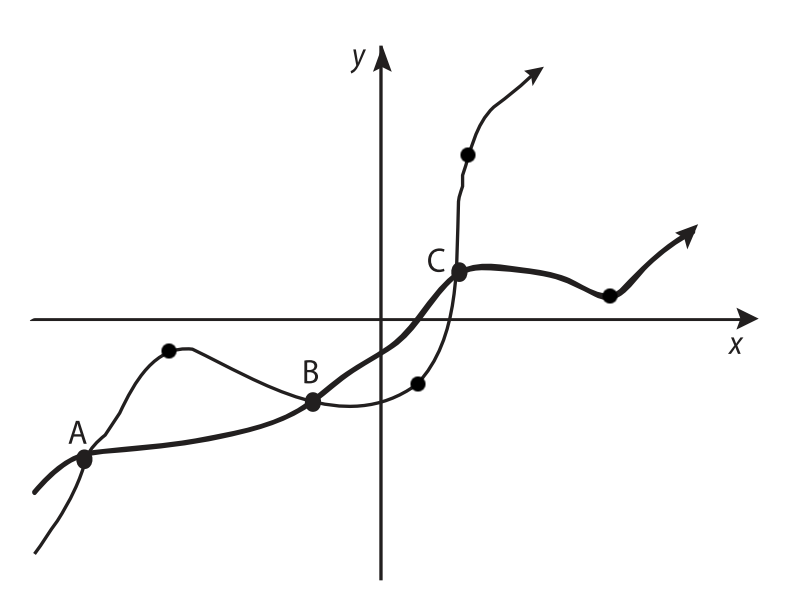
\includegraphics[width=60mm]{refs/coloc.png}
\caption{An example of co-location in 2D
space~\cite{Dodge:2008:TTM:1594710.1594716}.}
\end{figure}

Once a model for various agents as been built, this model can potentially be
used to produce a predictive model for agent location at a given day and time.
An underlying assumption of this analysis is that individual paths (and thus,
agents) will be easy to determine and separate from one another. This may not be
the case, as the analysis will show, and an auxiliary approach might be to
produce a ``best-guess'' of a given agent's path.

The most likely candidate algorithm to build this model will be a Hidden Markov
Model, as the data consists of many series of temporarily and geographically data
points, which may or may not be repeated over a greater time span. Specifically,
the goal will be to find periodic spatio-temporal patterns as described
in~\cite{laube2007movement}, and attempt to ``merge'' repeated patterns into a
single cohesive pattern, commonly referred to as a
\emph{thoroughfare}~\cite{Verhein06miningspatio-temporal} or more
conventionally, \emph{generalized sequential patterns}~\cite{Orellana2012672}.

\section{Evaluation Approach}
\label{sec:results}
Ideally, these results will show deterministic patterns in the sequence of
events which make up the paths of the agents, which will be easily identifiable
over a long period of time.  If the results do show a deterministic pattern, the
data will be used to build a model of the agent's behavior, specific to
geographic location, time of day, day of week, etc. These models will then be
analyzed for their effectiveness as well. This data will reveal and identify
interesting patterns or behaviors of the agents. The process of discovering
patterns in sequences of events is a well-studied field of artificial
intelligence~\cite{Dietterich85discoveringpatterns}. If the data does not show
such a deterministic pattern, it will be analyzed to show areas which might be
under-visited, and the analysis will be used to attempt to create artificial
agents which can be trained to develop the most efficient pattern based on the
historical data.

\section{Milestones}
Several milestones for the project are as follows:
\begin{itemize}
    \item \textbf{Mid-January:} Finalize data collection framework;
    \item \textbf{Feb 1}: Collect over 100K records;
    \item \textbf{Early Feb}: Geo-code all location data;
    \item \textbf{Early Feb}: Perform basic analysis of data (location frequency analysis, etc.);
    \item \textbf{Mid Feb}: Machine learning algorithm, introductory analysis;
    \item \textbf{Late Feb}: In-depth analysis based on preliminary results;
    \item \textbf{March 1}: Prepare final results, presentation and paper.
\end{itemize}

\bibliographystyle{IEEEtran}
\bibliography{ppa}

\end{document}
